\documentclass{standalone}
\usepackage{pgfplots}
\pgfplotsset{compat=1.16}
\begin{document}
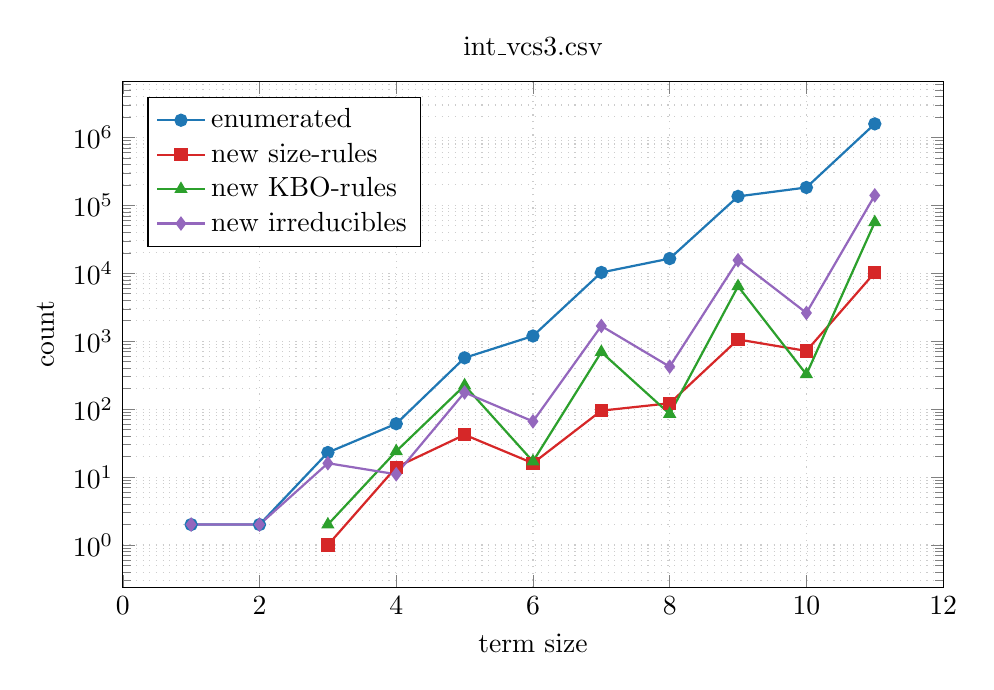
\begin{tikzpicture}
  \begin{axis}[
      width=12cm, height=8cm,
      xlabel={term size},
      ylabel={count},
      title={int\_vcs3.csv},
      ymode=log,
      grid=both,
      grid style={dotted, gray!40},
      legend pos=north west,
      legend cell align=left,
      mark size=2pt,
    ]
    \definecolor{cenumerated}{HTML}{1f77b4}
    \addplot[color=cenumerated, mark=*, thick] coordinates {(1,2) (2,2) (3,23) (4,61) (5,569) (6,1193) (7,10276) (8,16455) (9,135343) (10,183054) (11,1580324)};
    \addlegendentry{enumerated}
    \definecolor{cnewsizerules}{HTML}{d62728}
    \addplot[color=cnewsizerules, mark=square*, thick] coordinates {(1,0) (2,0) (3,1) (4,14) (5,42) (6,16) (7,95) (8,122) (9,1060) (10,719) (11,10244)};
    \addlegendentry{new size-rules}
    \definecolor{cnewkborules}{HTML}{2ca02c}
    \addplot[color=cnewkborules, mark=triangle*, thick] coordinates {(1,0) (2,0) (3,2) (4,24) (5,223) (6,17) (7,692) (8,85) (9,6429) (10,325) (11,56205)};
    \addlegendentry{new KBO-rules}
    \definecolor{cnewirreducibles}{HTML}{9467bd}
    \addplot[color=cnewirreducibles, mark=diamond*, thick] coordinates {(1,2) (2,2) (3,16) (4,11) (5,176) (6,66) (7,1676) (8,422) (9,15558) (10,2607) (11,140029)};
    \addlegendentry{new irreducibles}
  \end{axis}
\end{tikzpicture}
\end{document}
